\documentclass[11pt, oneside]{article}   	% use "amsart" instead of "article" for AMSLaTeX format
\usepackage{geometry}                		% See geometry.pdf to learn the layout options. There are lots.
\geometry{a4paper, total={6.8in, 8.5in}}
\usepackage{fancyhdr}
\usepackage{amsmath}
\usepackage{amssymb}
\usepackage{graphicx}				% Use pdf, png, jpg, or eps§ with pdflatex; use eps in DVI mode
\graphicspath{ {./} }
\usepackage{enumitem}
\usepackage{float}

\begin{document}
\pagestyle{fancy}
\fancyhead{}
\fancyhead[LO]{\textbf{CSE 5370}\\\textbf{BIO INFORMATICS}}
\fancyhead[RO]{\textbf{Sanjana Reddy Thigulla}\\1002142811}
\fancyhead[CO]{\LARGE{\textbf{Homework-2}}}

\begin{enumerate}
\item 

The original code uses the brute force method. It consists of two functions the overlap function and the  shortestCommonSuperstring function . The time complexity of the first function (overlap function ) is  $O(m^2)$ , where m is the maximum length of the string. The second function uses permutations functions so it has a time complexity of $O(n!)$ , where n is the number of strings and then it compares the superstrings to find the shortest one , its time complexity is $O(n)$. So the time complexity will be $O(n!*n*m^2)$.
\par
For the optimized version the same two functions have been used by optimizing them. The overlap function iterates m times where m is the length of the string so the time complexity will be $O(m)$. The second function no longer uses permutations instead it loops over the no of strings so the time complexity can be considered as $O(n^2)$ (lower order terms are ignored). So the time complexity will be $O(n^2 * m)$. This method is basically the greedy approach.
\par
The main idea was to remove the permutations because for larger inputs the original method wouldn’t be feasible. So using the greedy approach the number of comparisons have been reduced. Since all the permutations are not being checked the solution might not be the most efficient one but it effectively reduces the time complexity for large inputs. 
\\
\item 

\begin{enumerate}[label={2.\arabic*}]
  \item
 Using the given dataset generator for the UTA ID: 1002142811 a unique dataset of reads has been generated and stored in the text file “1002142811.txt”.
  \item
Considering k = 2, and reading in the “1002142811.txt” which contains the generated set of reads, a file named “kmers.txt” has been created which contains unique kmers of the reads.
  \item
For plotting the De Bruijn Graph the “kmers.txt” and “1002142811.txt” files have been read into the code and then networkx library(used for directed graphs) and matplotlib has been used.
\addtocounter{enumi}{1} % temporarily increase counter

\begin{figure}[H]
    \centering
    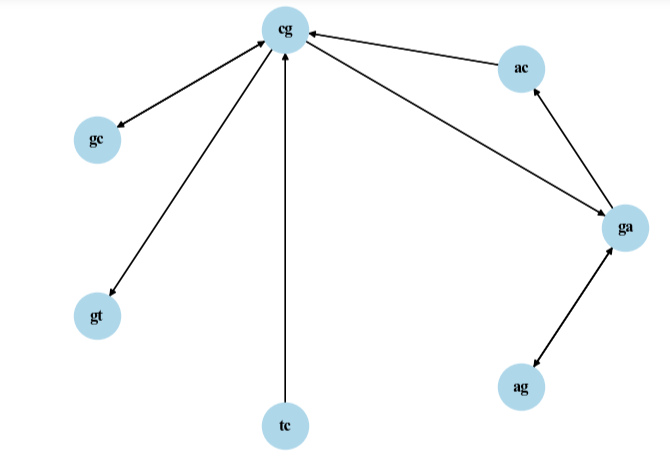
\includegraphics[width=0.6\textwidth]{debruijnplot}
    \caption{\footnotesize{De Bruijn Graph}}
    \label{fig:mesh1}
\end{figure}

\addtocounter{enumi}{-1} % reset counter
  \item There’s a Eulerian walk in the generated debruijn graph.
	\par
		For node cg: in-degree=3, out-degree=3 (balanced)
	\par
		For node ac: in-degree=1, out-degree=1 (balanced)
	\par
		For node ga: in-degree=2, out-degree=2 (balanced)
	\par
		For node gc: in-degree=1, out-degree=1 (balanced)	
	\par
		For node ag: in-degree=1, out-degree=1 (balanced)
	\par
		For node tc: in-degree=0, out-degree=1 (semi-balanced)
	\par
		For node gt: in-degree=1, out-degree=0 (semi-balanced)
	\par
		A debruijn graph is said have a Eulerian walk if it is directed, connected and if and only if it has at most 2 semi-balanced nodes and all other nodes balanced. Hence the generated debruijn graph can be called as Eulerian.

\item Since the generated Debruijn graph has a Eulerian walk , the walk gives a genome sequence. 
\begin{verbatim}
tc->cg->ga->ag->ga->ac->cg->gc->cg->gt
\end{verbatim}
\par
The assembled genome sequence is 
\par
\begin{center}
 \LARGE\textbf{“tcgagacgcgt”}
\end{center}
\par

 

\end{enumerate}

\item Difficulty adjustment: 
\begin{itemize}
\item It took me almost 5 days to work on this assignment. (I worked for about 3-5 hours each day). 

\item The first question confused me a bit. I used greedy approach to optimize the code ( explained in one of the lectures) and I tried running the code by giving some strings as input but the original version and my optimized version produced different outputs because of less number of comparisons. 

\item For the second question I had to refer to the lecture notes as well as the internet (very few articles were available) to learn about the concept of debruijn graph, eulerian path and eulerian circle .


\end{itemize}



\end{enumerate}
\end{document}